\section{Results}
\label{sec:results}
\subsection{Study status and research questions}
This preliminary study evaluated the forecasting and pricing pipeline on the supplied synthetic dataset. RQ1 concerns booking-probability accuracy, RQ2 concerns the counterfactual revenue change from constrained prices, and RQ3 concerns off-peak occupancy and cancellations. Each question was assessed against the corresponding H1--H3 criterion defined in Methods. All models and policies are evaluated on the same final test period. The findings describe this simulator and the models fitted to it; no real aggregator records were used.

The analysis covers the full supplied synthetic dataset. These are measured simulation results, calculated with the accompanying code and retained in the saved outputs. These preliminary findings come from completed model runs on synthetic records; they are not projected outcomes or measurements from real bookings. The simulator's hidden parameters were excluded from training, model selection and price optimization. Only after fitting were these parameters used to check the final predictions and pricing policy against the known booking mechanism.

\subsection{Data actually used and deviations}
Table~\ref{tab:data} records the final analysis data. The 153,300 rows cover 730 days and 14 venues, with 15 offered slots per venue-day. The first 584 days form the development period, and the last 146 days form the test period. There are 31,888 booked and 90,752 unbooked development slots, compared with 9,988 booked and 20,672 unbooked test slots. Booking prevalence is 26.00\% and 32.58\%, respectively. The development period contained 3,187 cancellations among booked slots, and the test period contained 958. These correspond to 9.99\% and 9.59\% of bookings. Cancelled bookings remain positive examples for the booking target; the cancellation classifier models their later cancellation separately. No cancelled rows were discarded from the forecasting comparison. All 15 supplied columns are complete. The audit found no duplicate venue--time keys, nonpositive prices or missing prices, so all records were retained.

The generator reproduced the supplied CSV byte for byte with seed 2026. The same generation run recovered the hidden booking intercepts and price coefficients used in the simulator checks. Training windows expand across the development folds and therefore overlap. Adding their training and validation counts would count some observations more than once. Each validation fold is separated from its training observations by seven days. The held-out test observations occur from 8 April to 31 August 2026 and contain spring and summer dates only.


\begin{table}[t]
\centering
\caption{Final synthetic dataset and chronological validation sizes. Development includes all pre-test observations; fold windows overlap. Zero rows were removed.}
\label{tab:data}
\footnotesize
\setlength{\tabcolsep}{3.5pt}
\begin{tabular}{p{.46\columnwidth}p{.46\columnwidth}}
\toprule
Item & Value \\
\midrule
Source & Supplied synthetic booking simulator \\
Period & 2024-09-01 to 2026-08-31 \\
Venues / facility types & 14 / 4 \\
Rows before / after cleaning & 153,300 / 153,300 \\
Duplicates / invalid prices / missing cells & 0 / 0 / 0 \\
Development / test rows & 122,640 / 30,660 \\
Booked / unbooked development rows & 31,888 / 90,752 \\
Booked / unbooked test rows & 9,988 / 20,672 \\
Booking prevalence development / test & 26.00\% / 32.58\% \\
Fold 1 train / validation & 23,100 / 24,514 \\
Fold 2 train / validation & 47,614 / 24,472 \\
Fold 3 train / validation & 72,086 / 24,514 \\
Fold 4 train / validation & 96,600 / 24,570 \\
\bottomrule
\end{tabular}
\end{table}

Several parts of the original Methods were reduced or changed for this pilot. Real aggregator data and external weather observations are replaced by the supplied simulation. Hyperparameter search uses eight trials per learned candidate instead of 100. Training uses a CPU, and the LSTM has a fixed five- or eight-epoch search budget rather than early stopping. The neural comparison includes an LSTM but no Transformer. SARIMAX uses a restricted AIC order search and a fixed multi-step test forecast. The reported comparisons therefore cover the pilot search budget; the larger tuning study remains unfinished.

The price-response analysis uses past-only orthogonalized estimation. There are no real price interventions, instruments, difference-in-differences episodes or randomized customer experiments in these files. Leave-venue-out evaluation and the realized-weather comparison remain unperformed. The planned minimum detectable commercial revenue effect is also unavailable. No commercial partner supplied a cost threshold; zero is used for H2, while the cost and cancellation-penalty fractions remain simulation assumptions. 

\subsection{RQ1 Booking probability forecasts}


Mean validation log-loss was 0.5031 for LightGBM, 0.5137 for the LSTM and 0.5329 for logistic regression. LightGBM was selected before evaluating the held-out test period. Table~\ref{tab:main} reports the common test comparison. The selected model's Brier score was 0.1951, compared with 0.2107 for climatology, 0.2092 for logistic regression, 0.1954 for the LSTM and 0.2038 for SARIMAX. Its log-loss was 0.5747. All four fitted models had positive Brier skill relative to climatology.

The selected LightGBM configuration used 240 trees, a learning rate of 0.06824, seven leaves per tree and a minimum of 80 observations per leaf. The selected LSTM had 24 hidden units and eight training epochs, with a learning rate of 0.00597. Logistic regression used $C=0.00103$. The validation search selected these configurations before their performance on the test set was known.

For LightGBM and the LSTM, the main comparison uses predictions averaged across the five model seeds. The individual LSTM runs had a mean Brier score of 0.1962, with a standard deviation of 0.0003; their mean log-loss was 0.5772, with a standard deviation of 0.0006. LightGBM's fixed, deterministic configuration produced identical probability scores across the five recorded seeds. Sampling uncertainty is reported separately through the intervals in Table~\ref{tab:main}. Logistic regression was fitted once after tuning, and SARIMAX contributed one AIC-selected fit per venue.


\begin{table*}[t]
\centering
\caption{Main test results on 30,660 synthetic slots. Brackets give 95\% venue-week bootstrap intervals. All values are dimensionless. Lower Brier, log-loss and ECE are preferable; larger AUC and BSS are preferable. Calibration targets are slope 1 and intercept 0.}
\label{tab:main}
\footnotesize
\setlength{\tabcolsep}{3.5pt}
\begin{tabular}{lccccccc}
\toprule
Model & Brier [95\% CI] & Log-loss [95\% CI] & AUC & ECE & BSS & Slope & Intercept \\
\midrule
Climatology & 0.2107 [0.2058, 0.2155] & 0.6181 [0.6062, 0.6301] & 0.6453 & 0.0665 & 0.0000 & 0.6912 & 0.0388 \\
Logistic & 0.2092 [0.2053, 0.2128] & 0.6072 [0.5983, 0.6156] & 0.6355 & 0.0301 & 0.0071 & 0.7486 & -0.1628 \\
LightGBM & 0.1951 [0.1915, 0.1984] & 0.5747 [0.5665, 0.5823] & 0.6973 & 0.0043 & 0.0740 & 1.0385 & 0.0393 \\
LSTM & 0.1954 [0.1919, 0.1987] & 0.5753 [0.5671, 0.5830] & 0.6964 & 0.0038 & 0.0724 & 1.0010 & 0.0051 \\
SARIMAX & 0.2038 [0.2003, 0.2071] & 0.5957 [0.5878, 0.6032] & 0.6612 & 0.0152 & 0.0326 & 1.0516 & 0.0472 \\
\bottomrule
\end{tabular}
\end{table*}

The paired comparisons in Table~\ref{tab:tests} report the loss differences and the evidence from the planned statistical tests. LightGBM had lower Brier score and log-loss than climatology, logistic regression and SARIMAX, with Holm-adjusted $p=0.0040$ for each comparison after rounding. The differences against the LSTM were much smaller: $-0.0003$ in Brier score and $-0.0006$ in log-loss. Both paired intervals included zero, and their adjusted $p$-values were 0.1859 and 0.2369. Because the comparison with the LSTM did not establish lower loss, H1 was not satisfied.

The selected model's calibration slope was 1.0385, with a 95\% interval of 1.0019 to 1.0768; its intercept was 0.0393. The slope interval excluded one, so the calibration component of H1 also failed. Figure~\ref{fig:reliability} plots predicted and observed booking probabilities. The LSTM had ECE 0.0038, compared with 0.0043 for LightGBM. LightGBM remained the model selected by validation log-loss; test calibration was reported without changing that choice. All 14 selected venue-level SARIMAX fits reported optimizer convergence.


\begin{table*}[t]
\centering
\caption{Paired loss differences, LightGBM minus the named baseline. Negative values favour LightGBM. Intervals use 2,000 venue-week replicates; adjusted p-values apply Holm correction across eight tests.}
\label{tab:tests}
\footnotesize
\setlength{\tabcolsep}{3.5pt}
\begin{tabular}{llrrr}
\toprule
Baseline & Loss & Difference & 95\% CI & Adjusted $p$ \\
\midrule
Climatology & Brier & -0.0156 & [-0.0180, -0.0132] & 0.0040 \\
Climatology & Log-loss & -0.0434 & [-0.0500, -0.0370] & 0.0040 \\
Logistic & Brier & -0.0141 & [-0.0154, -0.0129] & 0.0040 \\
Logistic & Log-loss & -0.0325 & [-0.0355, -0.0296] & 0.0040 \\
LSTM & Brier & -0.0003 & [-0.0007, 0.0001] & 0.1859 \\
LSTM & Log-loss & -0.0006 & [-0.0015, 0.0004] & 0.2369 \\
SARIMAX & Brier & -0.0087 & [-0.0097, -0.0078] & 0.0040 \\
SARIMAX & Log-loss & -0.0210 & [-0.0235, -0.0188] & 0.0040 \\
\bottomrule
\end{tabular}
\end{table*}

\begin{figure}[t]
\centering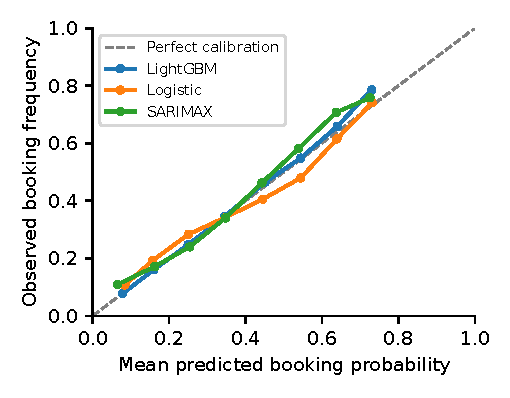
\includegraphics[width=\columnwidth]{reliability.pdf}
\caption{Test-set reliability on synthetic slots. Both axes are dimensionless probabilities. Points show ten equal-width probability bins with at least 20 observations; the dashed diagonal indicates equal predicted and observed booking rates.}
\label{fig:reliability}
\end{figure}


\begin{figure*}[t]
\centering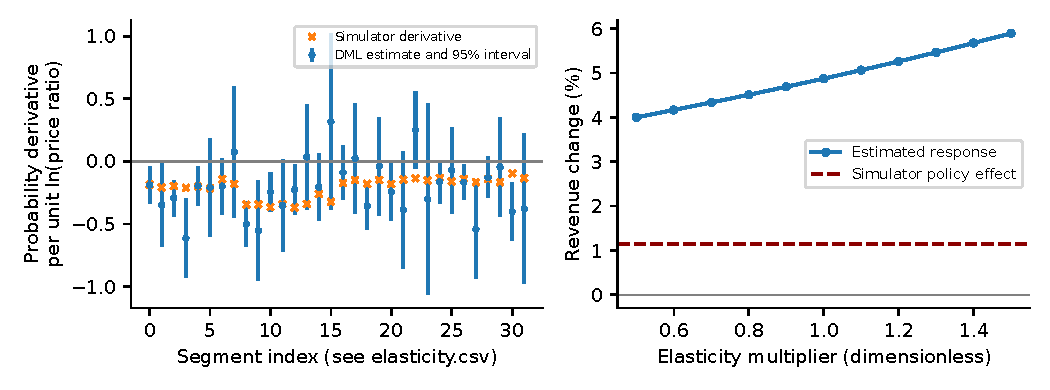
\includegraphics[width=.98\textwidth]{elasticity_sensitivity.pdf}
\caption{Price-response diagnostics on synthetic data. Left: estimated segment probability derivatives with 95\% clustered intervals and simulator average local derivatives; the segment index follows the saved elasticity table. Right: revenue change for the fixed chosen policy when estimated elasticities are multiplied by 0.5--1.5. The horizontal dashed line gives the known simulator effect for that policy.}
\label{fig:elasticity}
\end{figure*}


At the venue-day level, the LSTM had MAE 1.371 bookings per day and WAPE 28.05\%, compared with 1.378 and 28.19\% for LightGBM. Table~\ref{tab:secondary} gives the remaining values. These aggregated measures were not assessed with a separate paired test, so the reported ordering is descriptive. Aggregation changes the scored quantity from individual booking probabilities to the expected number of bookings across each venue-day.

\subsection{RQ2 Price response and counterfactual revenue}
Cross-fitting supplied 98,070 residual observations across 32 segments. Segment counts ranged from 531 to 7,195. The residual-to-observed log-price variance ratio ranged from 0.812 to 0.867, and all 32 segments met the sample-size and residual-variance thresholds. Five estimated probability derivatives were positive, although the simulator's local booking response to price was negative. Figure~\ref{fig:elasticity} shows the estimates and their intervals in the segment order retained in the accompanying CSV.

Against the simulator's average local derivative, the mean absolute discrepancy was 0.1647 for the orthogonalized estimate and 0.3125 for the naive estimate. The simulator derivative lay inside 29 of the 32 estimated intervals, or 90.6\%. This check compares the fitted partially linear coefficient with the average local derivative of the nonlinear generator. The two quantities have different statistical targets, so interval overlap is reported as a diagnostic.

The training revenue normalization factor was 1.0341. On test data, modeled revenue at historical prices divided by observed booking revenue was 0.9882. The corresponding modeled booking rate was 32.38\%, compared with the observed 32.58\%. The policy changed prices for 97.57\% of slots, and the mean recommended-to-historical price ratio was 1.0358. There were 20,259 price increases, 9,655 decreases and 746 unchanged prices, counting differences smaller than one millionth of a currency unit as unchanged. The no-change option remained available in the optimization. These recommendations were evaluated offline and were not implemented with customers. The demand diagnostics use the fitted price-response layer; checks using the generator's hidden booking probabilities are reported separately.

Table~\ref{tab:policy} reports a modeled revenue change of 4.87\%, with a 95\% interval of 3.28 to 6.79\%. Its lower bound exceeded the zero threshold, so the estimated-demand calculation satisfied H2. Evaluating exactly the same recommended prices under the simulator's known booking function gave 1.15\%. That value was below the lower endpoint of the estimated interval. The absolute difference between estimated and simulator revenue changes was 3.73 percentage points. No realized commercial revenue increase was observed.


\begin{table}[t]
\centering
\caption{Recommended minus historical policy on the same synthetic test slots. Estimated intervals combine venue-week resampling and 1,000 elasticity draws. The simulator column evaluates the fixed chosen prices using the known mechanism and is a deterministic expectation, not observed customer revenue.}
\label{tab:policy}
\footnotesize
\setlength{\tabcolsep}{3.5pt}
\begin{tabular}{lrrr}
\toprule
Outcome & Estimate & 95\% CI & Simulator \\
\midrule
Revenue change (\%) & 4.87 & [3.28, 6.79] & 1.15 \\
Utilization change (pp) & 0.56 & [0.02, 1.16] & -0.56 \\
Off-peak change (pp) & -0.31 & [-0.94, 0.33] & -0.92 \\
Cancellation change (pp) & -0.51 & [-0.69, -0.32] & -0.94 \\
\bottomrule
\end{tabular}
\end{table}

With the chosen policy held fixed, multiplying all estimated elasticities by a common factor from 0.5 to 1.5 produced revenue changes from 4.00\% to 5.90\%. Figure~\ref{fig:elasticity} shows the complete sensitivity curve. The calculated changes remained positive across the tested factors; no break-even factor was observed in this interval. The horizontal simulator value evaluates the same policy under its full known response, whereas the curve changes one shared multiplier in the estimated response model.

\subsection{RQ3 Off-peak occupancy and cancellations}
Under estimated demand, overall utilization changed by 0.56 percentage points, with an interval of 0.02 to 1.16. The simulator evaluation gave -0.56 percentage points for the same prices. The estimated response predicted an increase, while the simulator response gave a decrease in overall utilization. Off-peak occupancy changed by -0.31 percentage points under estimated demand, with an interval of -0.94 to 0.33; the corresponding simulator change was -0.92 percentage points.

The estimated cancellation-rate change was -0.51 percentage points, with an interval of -0.69 to -0.32. The training-derived non-inferiority margin was 0.75 percentage points, and the estimated upper bound was below that margin. The cancellation condition passed, but the lower bound for off-peak occupancy did not exceed zero. H3 was therefore not satisfied. Both cancellation rates use expected bookings as the denominator. Offered slots without a booking are excluded from that denominator.


\subsection{Additional analyses and observed errors}
Removing the four weather variables from every covariate step increased LightGBM's Brier score from 0.1951 to 0.1974 and log-loss from 0.5747 to 0.5806. The paired Brier difference was 0.0023, with a 95\% interval of 0.0017 to 0.0029. The corresponding log-loss interval was 0.0044 to 0.0073. The ablation was evaluated separately from the eight primary tests. Its bootstrap intervals are descriptive, and no multiplicity-adjusted significance is claimed for these additional comparisons.

Figure~\ref{fig:groups} compares observed and predicted booking rates by facility type. Football had an observed rate of 34.25\% and a predicted rate of 32.97\%, the largest absolute rate discrepancy among the four types. Swimming had the highest group Brier score, 0.2091; tennis had the lowest, 0.1845. Booking prevalence differs across these groups. The scores describe each group's prediction errors without establishing a controlled comparison of facility difficulty. The saved group table includes denominators, booked counts and log-loss for every type.

A further descriptive error check examined the 1,875 test slots with predicted booking probability of at least 0.60. Their mean prediction was 65.74\%, and 1,280 were booked, an observed rate of 68.27\%. The remaining 595 slots were unbooked despite receiving predictions above that threshold. The 0.60 threshold was used for this descriptive error check only. It had no role in model selection or recalibration.

The seasonal breakdown contains 11,340 spring slots and 19,320 summer slots. LightGBM's Brier score was 0.1793 in spring and 0.2043 in summer; the observed booking rates were 27.72\% and 35.43\%. No autumn or winter test scores were available. The test period therefore provides two seasonal groups, while all four seasons occur in the development data.

Several parts of the pipeline did not meet the specified checks. LightGBM's loss advantage over the LSTM was not supported, five estimated price derivatives were positive, and the simulator revenue effect fell outside the estimated interval. Estimated and simulator utilization changes also had opposite signs. H1 and H3 did not satisfy all their conditions. The selected model, price policy, test set and success thresholds were kept fixed after these outcomes were observed. Their causes and implications are left for the Discussion.


\begin{table}[t]
\centering
\caption{Venue-day errors after summing slot probabilities. MAE is measured in bookings per venue-day and WAPE is a percentage. These secondary measures use the same test slots as the main probability comparison.}
\label{tab:secondary}
\footnotesize
\setlength{\tabcolsep}{3.5pt}
\begin{tabular}{lrr}
\toprule
Model & MAE (bookings/day) & WAPE (\%) \\
\midrule
Climatology & 1.810 & 37.04 \\
Logistic & 1.677 & 34.32 \\
LightGBM & 1.378 & 28.19 \\
LSTM & 1.371 & 28.05 \\
SARIMAX & 1.400 & 28.64 \\
\bottomrule
\end{tabular}
\end{table}

\begin{figure}[t]
\centering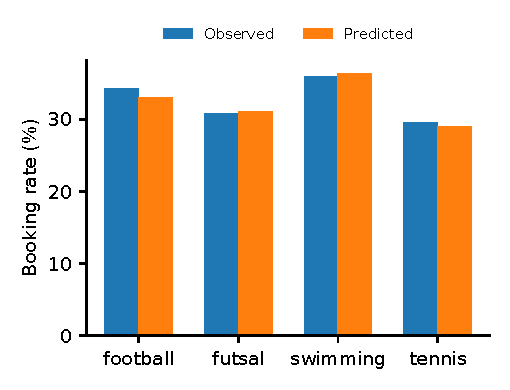
\includegraphics[width=\columnwidth]{group_errors.pdf}
\caption{Observed and LightGBM-predicted booking rates by synthetic facility type on the common test period. Football and futsal each have 8,760 slots; swimming and tennis each have 6,570. Bars show rates as percentages of offered slots.}
\label{fig:groups}
\end{figure}


\subsection{Reproducibility}
Repository publication is pending. The complete code, data, results and manuscript source accompany this article in the submission archive.

The run used Python 3.12.14, NumPy 2.3.5, pandas 2.2.3, scikit-learn 1.8.0, SciPy 1.17.0, LightGBM 4.7.0, Optuna 5.0.0, PyTorch 2.14.1{+}cpu and statsmodels 0.15.0. The execution platform was Linux on an AMD EPYC 9V74 80-Core Processor, with 9 logical CPUs visible and two computation threads configured for the fitted models. No GPU was used. A clean analysis run took approximately 6.0 minutes in this environment, excluding package installation and manuscript compilation; runtime on another computer will differ.

The generator and tuning seeds were 2026, model seeds were 0--4, the forecast bootstrap seed was 2026, and the combined elasticity and policy bootstrap used seed 123. The package records split boundaries, search trials, selected hyperparameters, per-seed scores, test predictions, paired tests, elasticity estimates and simulator checks. It includes a script that checks reported scores against saved predictions and verifies the test membership, temporal gaps, price grid and revenue arithmetic. All tabular values and vector figures in this section can be regenerated from the supplied data and code.
\FloatBarrier
